% \begin{chapter}*{}

% \aosafigure{../images/backmatter/making.pdf}{}{fig.making.making}
\thispagestyle{empty}

\sffamily

%\Large You May Also Enjoy\ldots
\Large Tambi�n Puedes Disfrutar\ldots

\normalsize

\begin{figure}[h!]
\centering
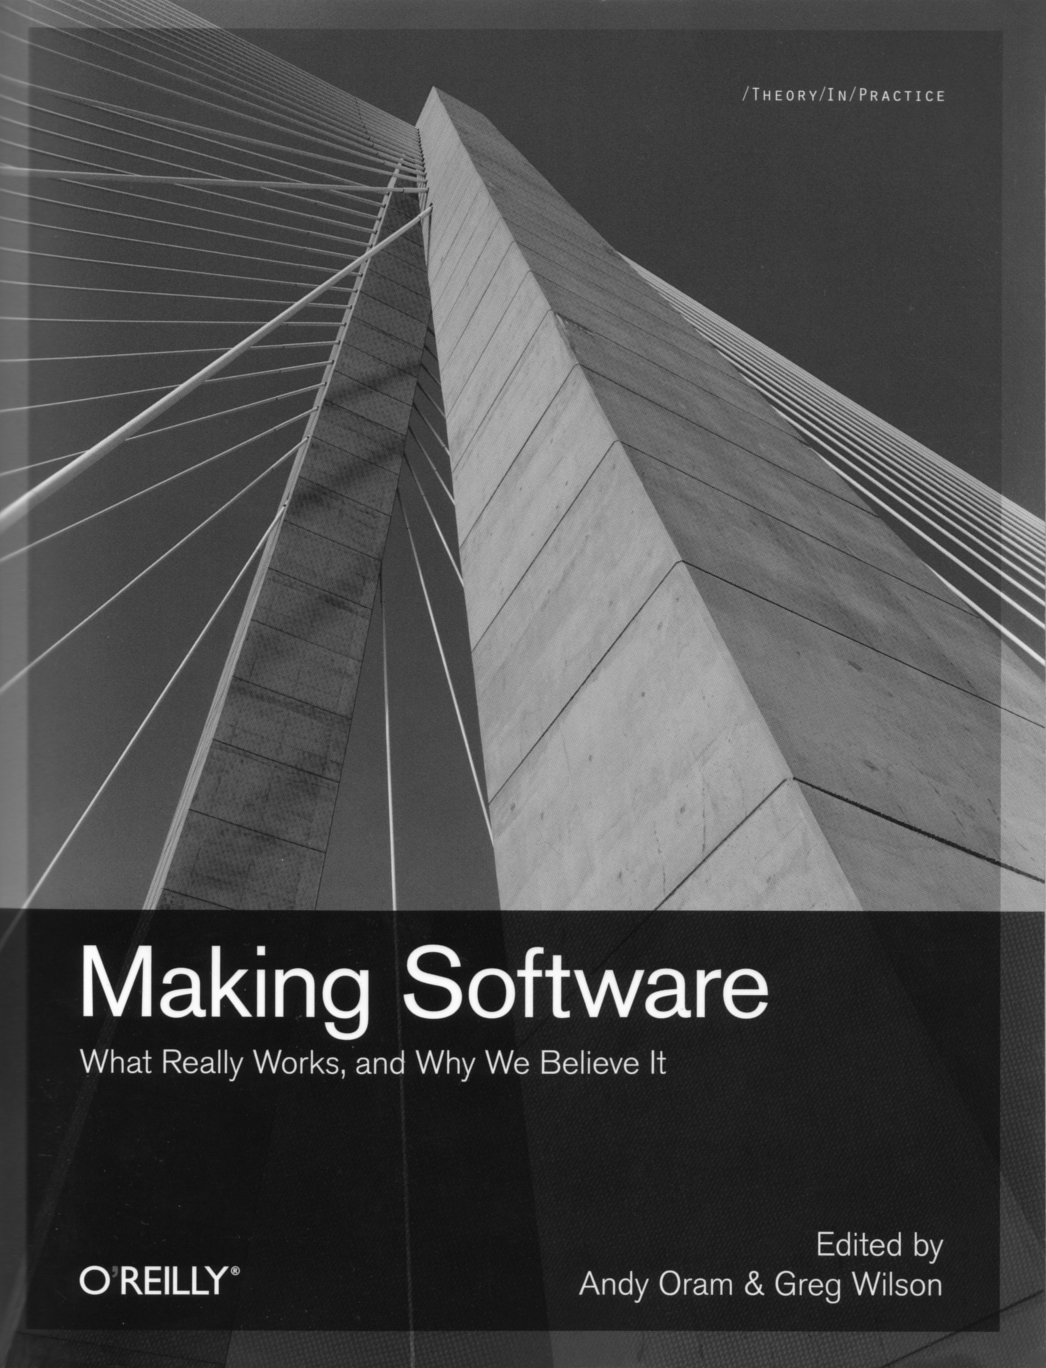
\includegraphics[width=250pt]{../images/backmatter/making.pdf}
\end{figure}

%Many claims are made about how certain tools, technologies, and
%practices improve software development. But which are true, and which
%are merely wishful thinking? In \emph{Making Software}, leading
%researchers and practitioners present chapter-length summaries of key
%empirical findings in software engineering, and answer questions like:
Se hacen muchas afirmaciones acerca de c�mo ciertas herramientas, tecnolog�as
y pr�cticas mejoran el desarrollo del software. Pero cu�les son ciertas
y cu�les son s�lo buenos deseos? En \emph{Making Software}, investigadores y
profesionales l�deres presentan res�menes por cap�tulo acerca de importantes
hallazgos emp�ricos en ingenier�a de software y responden a preguntas tales como:

\vspace{-0.1cm}

\begin{aosaitemize}

%\item Are some programmers really ten times more productive than others?
\item �Realmente algunos programadores son diez veces m�s productivos que otros?

%\item Does writing tests first help you develop better code faster?
\item �Escribir tests al principio ayuda a desarrollar mejor c�digo y m�s r�pido?

%\item Can code metrics predict the number of bugs in a piece of software?
\item �Pueden las m�tricas de c�digo predecir la cantidad de errores en un componente de software?

%\item Does using design patterns actually make software better?
\item �Utilizar patrones de dise�o realmente hace mejor al software?

%\item What effect does personality have on pair programming?
\item �C�mo afecta la personalidad en la programaci�n en parejas (pair-programming)?

%\item What matters more: how far apart people are geographically, or how far apart they are in the org chart?
\item �Qu� es m�s importante: qu� tan lejos est�n las personas geogr�ficamente, o qu� tan lejos est�n en
el cuadro organizacional?

\end{aosaitemize}

\vspace{-0.2cm}

\setlength{\parskip}{0.15cm}

%\noindent As with \emph{The Architecture of Open Source Applications}, royalties
%from \emph{Making Software} will be donated to Amnesty International.
\noindent As� como en \emph{La Arquitectura de las Aplicaciones de C�digo Libre}, las ganancias
de \emph{Making Software} (Haciendo Software) ser�n donadas a Amnist�a Internacional.

\noindent \emph{Making Software: What Really Works, and Why We Believe It} \\
editado por Andy Oram and Greg Wilson \\
O'Reilly Media, 2010, 978-0596808327 \\
\url{http://oreilly.com/catalog/9780596808303}

\normalfont

\pagebreak
\thispagestyle{empty}

